% !TeX root = ../../main.tex
\newpage
\section{Anotator danych}

Każdy obraz, aby mógł służyć za rekord treningowy, musi zostać zaanotowany - to znaczy musi zostać na nim oznaczony obszar kortu.
Dotyczy to zarównu sztucznie wygenerowanych danych, obrazów pochodzących od firmy \blue{}, jak i obrazów pochodzących z Internetu.
Dlatego też jednym z niezbędnych elementów aplikacji jest anotator danych, który został wykorzystany podczas konstruowania zbiorów danych \textit{low} oraz \textit{high}, opisanych w rozdziale \myrefx{sec:zbiory}.

Wykorzystano otwarto źródłowy program \textit{VGG Image Annotator} \cite{dutta2016via} \cite{dutta2019vgg}, napisany w \textit{HTML}, \textit{JavaScript} i \textit{CSS}, bez żadnych dodatkowych zależności.
Dzięki temu do uruchomienia programu nie potrzebne jest nic poza przeglądarką internetową.
Na Rysunku \myfigrefx{fig:via} przedstawiono zrzut ekranu uruchomionego anotatora danych, podczas anotacji jednego z obrazów zbioru  \textit{high}.

\vspace{1cm}

\begin{figure}[!htb]
  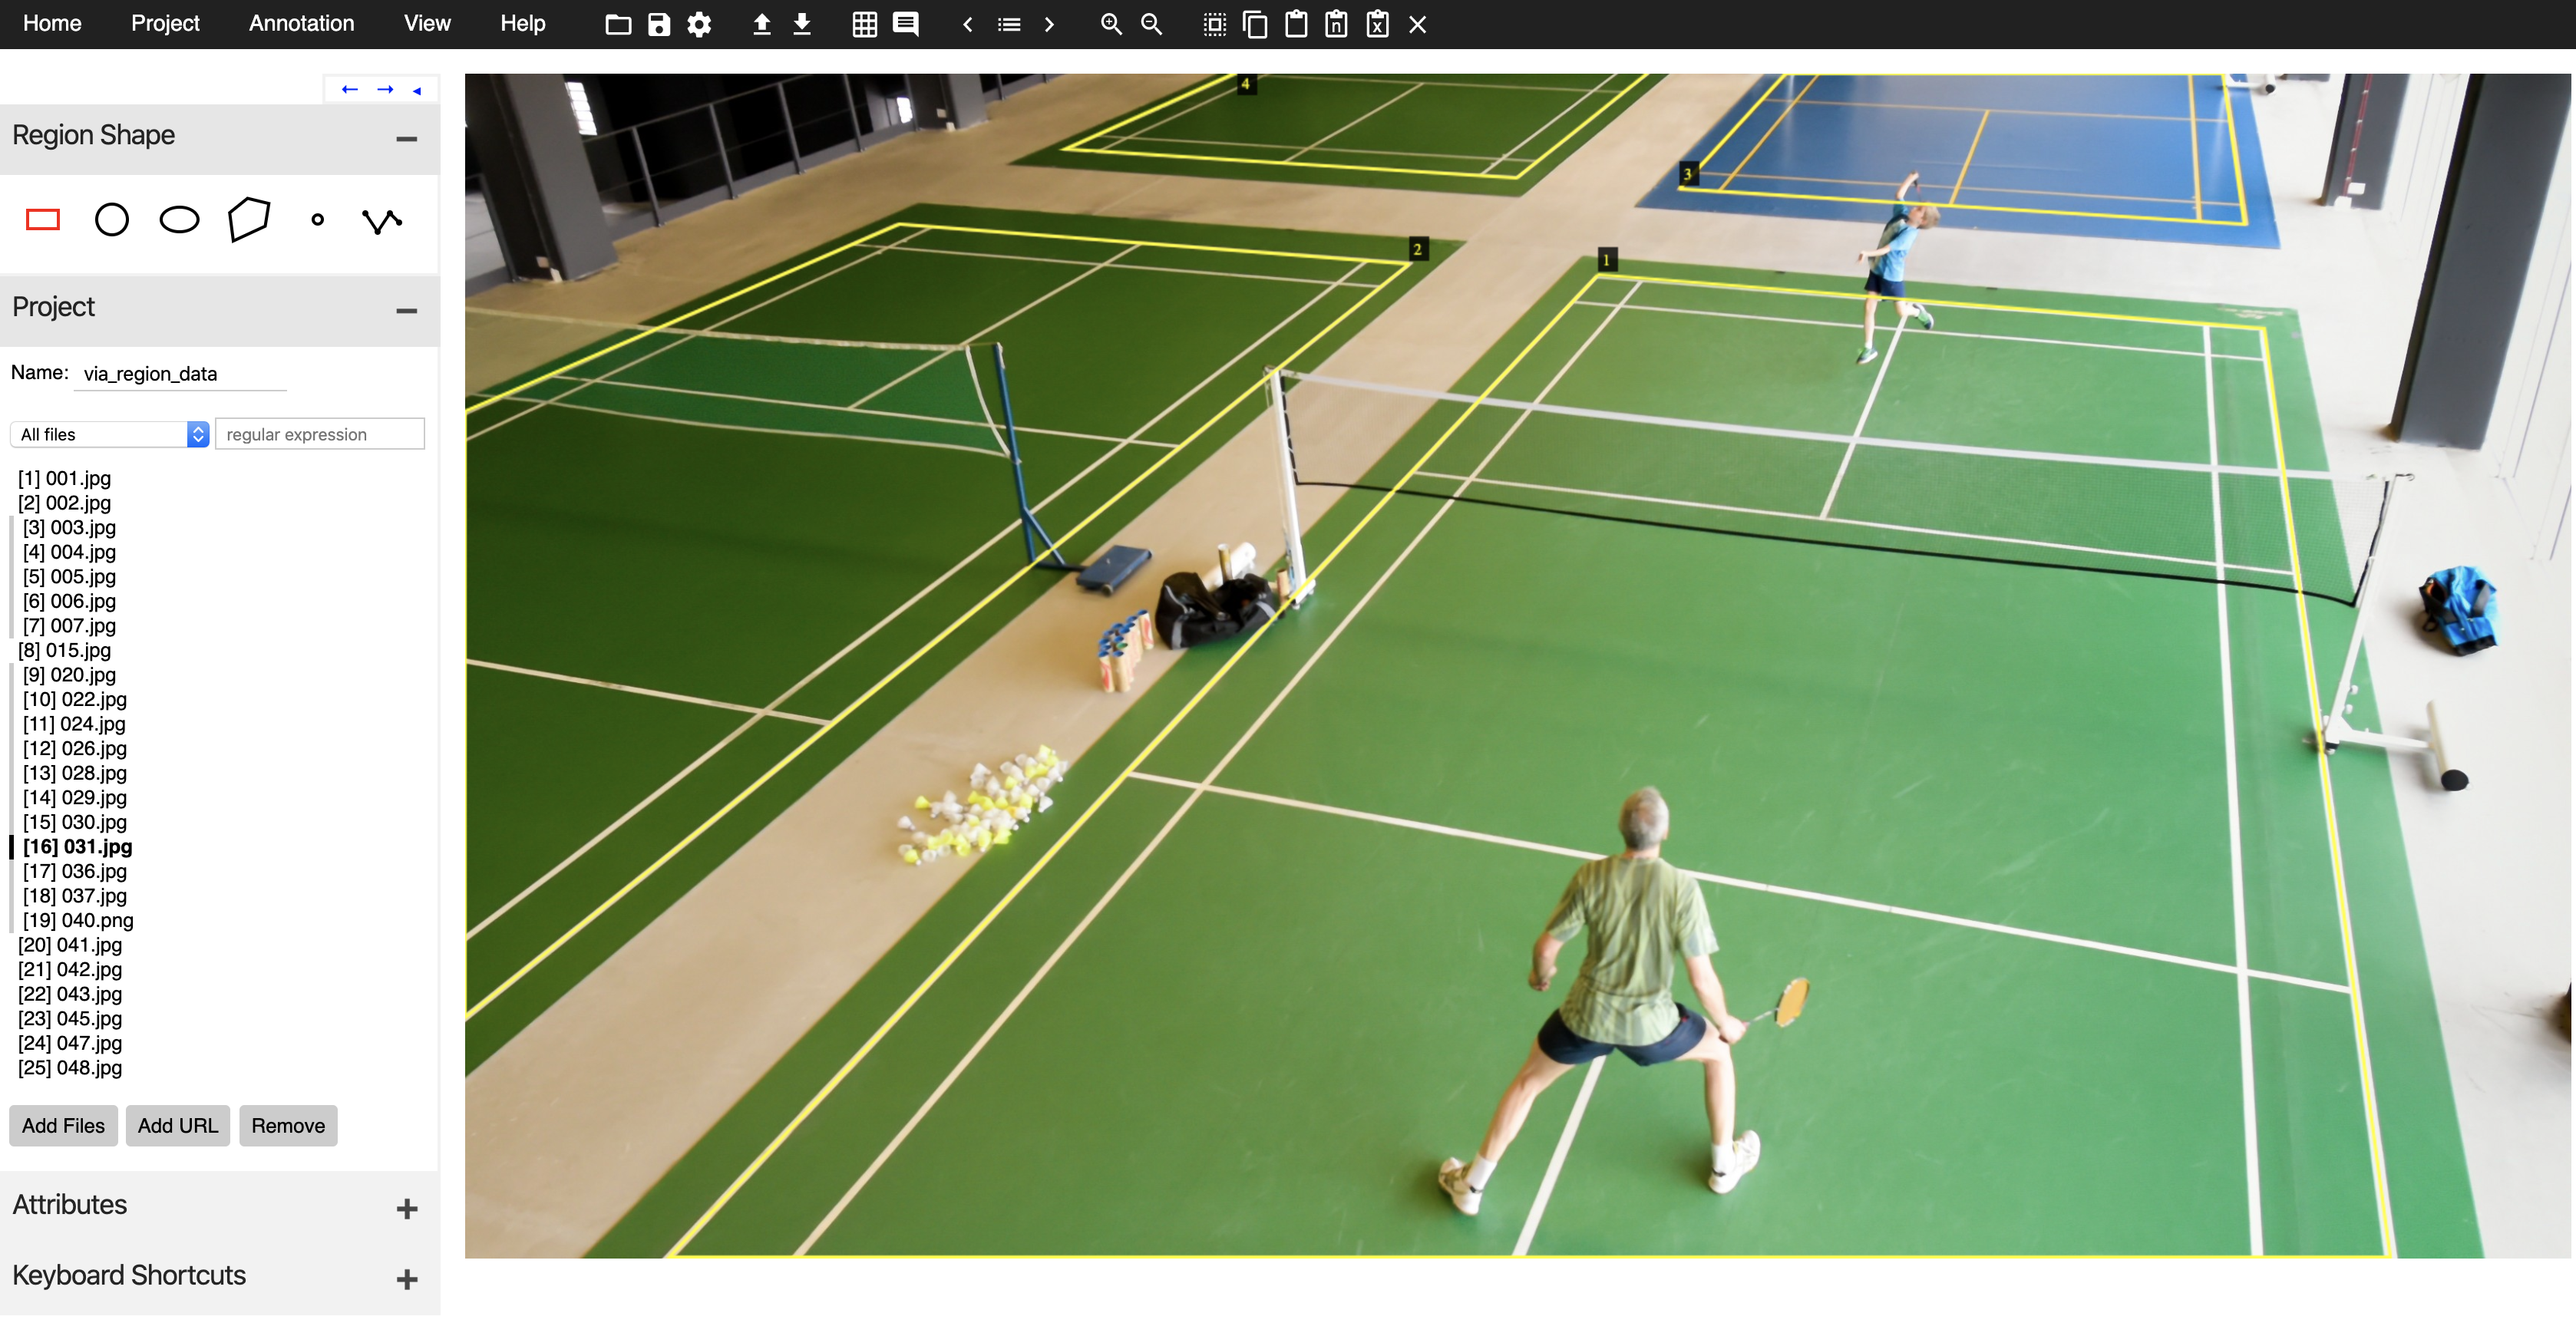
\includegraphics[width=\linewidth]{./via.png}
    \caption{Zrzut ekranu uruchomionego anotatora danych}
    \label{fig:via}
\end{figure}
